\documentclass[frenchb, paper=a4, fontsize=11pt]{scrartcl}

\usepackage[utf8x]{inputenc}
\usepackage[T1]{fontenc}
\usepackage{lmodern}

\usepackage{ifthen}
\usepackage{url}


\usepackage{multirow}

% Color
% cfr http://en.wikibooks.org/wiki/LaTeX/Colors
\usepackage{color}
\usepackage[usenames,dvipsnames,svgnames,table]{xcolor}
\definecolor{dkgreen}{rgb}{0.25,0.7,0.35}
\definecolor{dkred}{rgb}{0.7,0,0}

\newcommand{\matlab}{\textsc{Matlab}}

% Math symbols
\usepackage{amsmath}
\usepackage{amssymb}
\usepackage{amsthm}
\DeclareMathOperator*{\argmin}{arg\,min}
\DeclareMathOperator*{\argmax}{arg\,max}


% Sets
\newcommand{\Z}{\mathbb{Z}}
\newcommand{\R}{\mathbb{R}}
\newcommand{\Rn}{\R^n}
\newcommand{\Rnn}{\R^{n \times n}}
\newcommand{\C}{\mathbb{C}}
\newcommand{\K}{\mathbb{K}}
\newcommand{\Kn}{\K^n}
\newcommand{\Knn}{\K^{n \times n}}

% Unit vectors
\usepackage{esint}
\usepackage{esvect}
\newcommand{\kmath}{k}
\newcommand{\xunit}{\hat{\imath}}
\newcommand{\yunit}{\hat{\jmath}}
\newcommand{\zunit}{\hat{\kmath}}
\newcommand{\uunit}{\hat{\umath}}

% rot & div & grad & lap
\DeclareMathOperator{\newdiv}{div}
\newcommand{\divn}[1]{\nabla \cdot #1}
\newcommand{\rotn}[1]{\nabla \times #1}
\newcommand{\grad}[1]{\nabla #1}
\newcommand{\gradn}[1]{\nabla #1}
\newcommand{\lap}[1]{\nabla^2 #1}


% Elec
\newcommand{\B}{\vec B}
\newcommand{\E}{\vec E}
\newcommand{\EMF}{\mathcal{E}}
\newcommand{\perm}{\varepsilon} % permittivity

\newcommand{\bigoh}{\mathcal{O}}
\newcommand\eqdef{\triangleq}

\DeclareMathOperator{\newdiff}{d} % use \dif instead
\newcommand{\dif}{\newdiff\!}
\newcommand{\fpart}[2]{\frac{\partial #1}{\partial #2}}
\newcommand{\ffpart}[2]{\frac{\partial^2 #1}{\partial #2^2}}
\newcommand{\fdpart}[3]{\frac{\partial^2 #1}{\partial #2\partial #3}}
\newcommand{\fdif}[2]{\frac{\dif #1}{\dif #2}}
\newcommand{\ffdif}[2]{\frac{\dif^2 #1}{\dif #2^2}}
\newcommand{\constant}{\ensuremath{\mathrm{cst}}}

\usepackage{siunitx}

\usepackage{tikz}
\usepackage{tikz-3dplot}

\usepackage{pgfplots}
\usepackage{lmodern}
%\usepackage[protrusion=true,expansion=true]{microtype}
\usepackage{xspace}

\usepackage{babel}
% Listing
% always put it after babel
% http://tex.stackexchange.com/questions/100717/code-in-lstlisting-breaks-document-compile-error
\usepackage{listings}

\definecolor{mygreen}{rgb}{0,0.6,0}
\definecolor{mygray}{rgb}{0.5,0.5,0.5}
\definecolor{mymauve}{rgb}{0.58,0,0.82}
\lstset{ %
  language=Matlab,
  backgroundcolor=\color{white},   % choose the background color; you must add \usepackage{color} or \usepackage{xcolor}
  basicstyle=\footnotesize,        % the size of the fonts that are used for the code
  breakatwhitespace=false,         % sets if automatic breaks should only happen at whitespace
  breaklines=true,                 % sets automatic line breaking
  captionpos=b,                    % sets the caption-position to bottom
  commentstyle=\color{mygreen},    % comment style
  deletekeywords={...},            % if you want to delete keywords from the given language
  escapeinside={\%*}{*)},          % if you want to add LaTeX within your code
  extendedchars=true,              % lets you use non-ASCII characters; for 8-bits encodings only, does not work with UTF-8
  frame=single,	                   % adds a frame around the code
  keepspaces=true,                 % keeps spaces in text, useful for keeping indentation of code (possibly needs columns=flexible)
  keywordstyle=\color{blue},       % keyword style
  otherkeywords={*,...},           % if you want to add more keywords to the set
  numbers=none,                    % where to put the line-numbers; possible values are (none, left, right)
  numbersep=5pt,                   % how far the line-numbers are from the code
  numberstyle=\tiny\color{mygray}, % the style that is used for the line-numbers
  rulecolor=\color{black},         % if not set, the frame-color may be changed on line-breaks within not-black text (e.g. comments (green here))
  showspaces=false,                % show spaces everywhere adding particular underscores; it overrides 'showstringspaces'
  showstringspaces=false,          % underline spaces within strings only
  showtabs=false,                  % show tabs within strings adding particular underscores
  stepnumber=2,                    % the step between two line-numbers. If it's 1, each line will be numbered
  stringstyle=\color{mymauve},     % string literal style
  tabsize=2,	                   % sets default tabsize to 2 spaces
  title=\lstname                   % show the filename of files included with \lstinputlisting; also try caption instead of title
}

\KOMAoptions{DIV=last}

\usepackage[top = 2.5 cm, bottom = 3 cm, left = 2.5 cm, right = 2.5 cm]{geometry}
\usepackage{hyperref}
\usepackage{todonotes}
\DeclareSIUnit{\rot}{rot}
\usepackage[makeroom]{cancel}

%%% Custom sectioning (sectsty package)
\usepackage{sectsty}								% Custom sectioning (see below)
\allsectionsfont{\scshape}						% Change font of al section commands

%%% Custom headers/footers (fancyhdr package)
\usepackage{fancyhdr}
\pagestyle{fancyplain}
\fancyhead{}										% No page header
\fancyfoot[L]{\small Groupe 1}					% You may remove/edit this line 
\fancyfoot[C]{}									% Empty
\fancyfoot[R]{\thepage}							% Pagenumbering
\renewcommand{\headrulewidth}{0pt}				% Remove header underlines
\renewcommand{\footrulewidth}{0pt}				% Remove footer underlines
\setlength{\headheight}{13.6pt}

%%% Equation and float numbering
\numberwithin{equation}{section}					% Equationnumbering: section.eq#
\numberwithin{figure}{section}					% Figurenumbering: section.fig#
\numberwithin{table}{section}						% Tablenumbering: section.tab#

%%% Maketitle metadata
\newcommand{\horrule}[1]{\rule{\linewidth}{#1}} 	% Horizontal rule

\title{
		%\vspace{-1in} 	
		\usefont{OT1}{bch}{b}{n}
		\normalfont \normalsize \textsc{Ecole polytechnique de Louvain} \\ [25pt]
		\horrule{0.5pt} \\[0.4cm]
		\large LINMA1510 - Automatique linéaire\\
		\huge Laboratoire 2 - Contrôle d'un moteur à courant continu \\
		\horrule{1.5pt} \\[0.5cm]
}
\author{
		\normalfont
		\textsc{Groupe 62}\\
      	Antoine Paris\hspace{0.6cm} Philippe Verbist \\	
       	\normalsize
        \today
}
\date{}

\begin{document}
\maketitle

\section{Identification du modèle}

\begin{equation}
	G(s) = \frac{K}{1+s\tau}
\end{equation}


%\begin{figure}[ht]
%	\centering
%	% This file was created by matlab2tikz.
%
%The latest updates can be retrieved from
%  http://www.mathworks.com/matlabcentral/fileexchange/22022-matlab2tikz-matlab2tikz
%where you can also make suggestions and rate matlab2tikz.
%
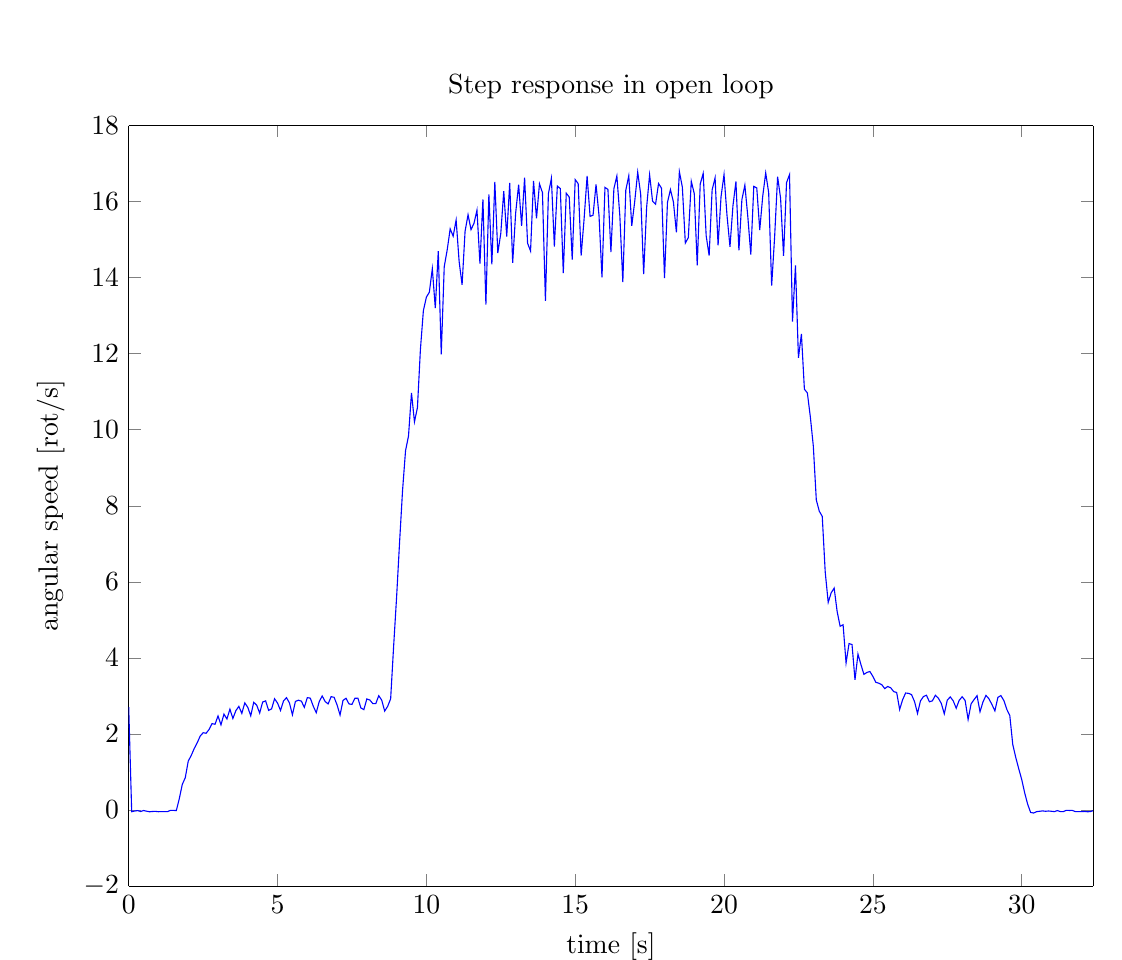
\begin{tikzpicture}

\begin{axis}[%
width=4.822in,
height=3.803in,
at={(0.809in,0.513in)},
scale only axis,
separate axis lines,
every outer x axis line/.append style={black},
every x tick label/.append style={font=\color{black}},
xmin=0,
xmax=32.4,
xlabel={time [s]},
every outer y axis line/.append style={black},
every y tick label/.append style={font=\color{black}},
ymin=-2,
ymax=18,
ylabel={angular speed [rot/s]},
axis background/.style={fill=white},
title={Step response in open loop}
]
\addplot [color=blue,solid,forget plot]
  table[row sep=crcr]{%
0	2.706113\\
0.1	-0.042591357\\
0.2	-0.026116869\\
0.3	-0.013444186\\
0.4	-0.038789552\\
0.5	-0.012176917\\
0.6	-0.029918674\\
0.7	-0.045125894\\
0.8	-0.037522284\\
0.9	-0.034987747\\
1	-0.043858626\\
1.1	-0.040056821\\
1.2	-0.041324089\\
1.3	-0.042591357\\
1.4	-0.008375112\\
1.5	-0.009642381\\
1.6	-0.012176917\\
1.7	0.30210562\\
1.8	0.674682482\\
1.9	0.849565492\\
2	1.286773\\
2.1	1.435043\\
2.2	1.616263\\
2.3	1.7658\\
2.4	1.943218\\
2.5	2.033194\\
2.6	2.019254\\
2.7	2.119368\\
2.8	2.272708\\
2.9	2.256233\\
3	2.472936\\
3.1	2.241026\\
3.2	2.522359\\
3.3	2.394365\\
3.4	2.652888\\
3.5	2.408305\\
3.6	2.613603\\
3.7	2.726389\\
3.8	2.541368\\
3.9	2.8189\\
4	2.701044\\
4.1	2.478005\\
4.2	2.834107\\
4.3	2.756804\\
4.4	2.551506\\
4.5	2.840444\\
4.6	2.870858\\
4.7	2.621206\\
4.8	2.659224\\
4.9	2.926618\\
5	2.812564\\
5.1	2.618672\\
5.2	2.868323\\
5.3	2.955765\\
5.4	2.816365\\
5.5	2.505885\\
5.6	2.855651\\
5.7	2.8886\\
5.8	2.864522\\
5.9	2.701044\\
6	2.955765\\
6.1	2.943092\\
6.2	2.731458\\
6.3	2.55911\\
6.4	2.849314\\
6.5	3.000119\\
6.6	2.853116\\
6.7	2.79102\\
6.8	2.98111\\
6.9	2.964636\\
7	2.764407\\
7.1	2.499548\\
7.2	2.882263\\
7.3	2.93929\\
7.4	2.79102\\
7.5	2.778347\\
7.6	2.93929\\
7.7	2.941825\\
7.8	2.683302\\
7.9	2.641482\\
8	2.921549\\
8.1	2.893669\\
8.2	2.799891\\
8.3	2.797356\\
8.4	3.006456\\
8.5	2.8886\\
8.6	2.602197\\
8.7	2.727657\\
8.8	2.924083\\
8.9	4.305405\\
9	5.600552\\
9.1	7.042703\\
9.2	8.403748\\
9.3	9.447976\\
9.4	9.837027\\
9.5	10.971231\\
9.6	10.208336\\
9.7	10.58218\\
9.8	12.113038\\
9.9	13.134455\\
10	13.485488\\
10.1	13.617284\\
10.2	14.23571\\
10.3	13.199086\\
10.4	14.698262\\
10.5	11.983777\\
10.6	14.286401\\
10.7	14.731211\\
10.8	15.282472\\
10.9	15.088581\\
11	15.515649\\
11.1	14.429602\\
11.2	13.808641\\
11.3	15.216575\\
11.4	15.653782\\
11.5	15.262196\\
11.6	15.428208\\
11.7	15.774172\\
11.8	14.368773\\
11.9	16.056772\\
12	13.287795\\
12.1	16.188568\\
12.2	14.351031\\
12.3	16.515523\\
12.4	14.647572\\
12.5	15.162082\\
12.6	16.274742\\
12.7	15.082244\\
12.8	16.487643\\
12.9	14.391584\\
13	15.701938\\
13.1	16.444556\\
13.2	15.364845\\
13.3	16.630844\\
13.4	14.906094\\
13.5	14.69953\\
13.6	16.54467\\
13.7	15.557469\\
13.8	16.468634\\
13.9	16.235457\\
14	13.39171\\
14.1	16.208844\\
14.2	16.610568\\
14.3	14.817386\\
14.4	16.407805\\
14.5	16.341907\\
14.6	14.116587\\
14.7	16.218983\\
14.8	16.117601\\
14.9	14.475224\\
15	16.576352\\
15.1	16.472436\\
15.2	14.581674\\
15.3	15.554935\\
15.4	16.671397\\
15.5	15.609427\\
15.6	15.642376\\
15.7	16.449625\\
15.8	15.634773\\
15.9	14.006335\\
16	16.372322\\
16.1	16.319097\\
16.2	14.674184\\
16.3	16.338106\\
16.4	16.672664\\
16.5	15.6221\\
16.6	13.884677\\
16.7	16.29882\\
16.8	16.676466\\
16.9	15.359776\\
17	16.004814\\
17.1	16.774045\\
17.2	16.19237\\
17.3	14.091242\\
17.4	15.85401\\
17.5	16.703078\\
17.6	16.007349\\
17.7	15.928778\\
17.8	16.473703\\
17.9	16.352046\\
18	13.987326\\
18.1	15.980736\\
18.2	16.314028\\
18.3	15.98834\\
18.4	15.188695\\
18.5	16.785451\\
18.6	16.378658\\
18.7	14.909896\\
18.8	15.050563\\
18.9	16.534532\\
19	16.208844\\
19.1	14.324419\\
19.2	16.459763\\
19.3	16.742364\\
19.4	15.102521\\
19.5	14.579139\\
19.6	16.305157\\
19.7	16.623241\\
19.8	14.8478\\
19.9	16.129007\\
20	16.710682\\
20.1	15.637307\\
20.2	14.812316\\
20.3	15.889493\\
20.4	16.526928\\
20.5	14.716004\\
20.6	16.049169\\
20.7	16.431883\\
20.8	15.596755\\
20.9	14.605752\\
21	16.400202\\
21.1	16.358382\\
21.2	15.253325\\
21.3	16.137877\\
21.4	16.753769\\
21.5	16.23419\\
21.6	13.788365\\
21.7	15.072106\\
21.8	16.654922\\
21.9	16.089721\\
22	14.571536\\
22.1	16.496514\\
22.2	16.708147\\
22.3	12.841717\\
22.4	14.31935\\
22.5	11.888732\\
22.6	12.519831\\
22.7	11.066276\\
22.8	10.967429\\
22.9	10.33633\\
23	9.569633\\
23.1	8.155363\\
23.2	7.858823\\
23.3	7.721958\\
23.4	6.254462\\
23.5	5.461153\\
23.6	5.712072\\
23.7	5.836264\\
23.8	5.220372\\
23.9	4.833856\\
24	4.873141\\
24.1	3.86693\\
24.2	4.378907\\
24.3	4.351027\\
24.4	3.424654\\
24.5	4.101375\\
24.6	3.823843\\
24.7	3.567855\\
24.8	3.618546\\
24.9	3.643891\\
25	3.51463\\
25.1	3.358756\\
25.2	3.335945\\
25.3	3.29666\\
25.4	3.192744\\
25.5	3.249771\\
25.6	3.214288\\
25.7	3.114173\\
25.8	3.091363\\
25.9	2.645284\\
26	2.901272\\
26.1	3.077423\\
26.2	3.068552\\
26.3	3.035603\\
26.4	2.851849\\
26.5	2.540101\\
26.6	2.870858\\
26.7	2.984912\\
26.8	3.019128\\
26.9	2.84678\\
27	2.870858\\
27.1	3.017861\\
27.2	2.943092\\
27.3	2.802426\\
27.4	2.53123\\
27.5	2.8886\\
27.6	2.976041\\
27.7	2.872125\\
27.8	2.676966\\
27.9	2.884798\\
28	2.979843\\
28.1	2.880996\\
28.2	2.381693\\
28.3	2.79102\\
28.4	2.905074\\
28.5	3.007723\\
28.6	2.584455\\
28.7	2.842978\\
28.8	3.014059\\
28.9	2.92535\\
29	2.775813\\
29.1	2.608534\\
29.2	2.962101\\
29.3	3.010257\\
29.4	2.880996\\
29.5	2.647819\\
29.6	2.48941\\
29.7	1.725248\\
29.8	1.386887\\
29.9	1.087812\\
30	0.806478374\\
30.1	0.454177811\\
30.2	0.1551025\\
30.3	-0.062867651\\
30.4	-0.078074871\\
30.5	-0.042591357\\
30.6	-0.032453211\\
30.7	-0.022315064\\
30.8	-0.032453211\\
30.9	-0.024849601\\
31	-0.032453211\\
31.1	-0.041324089\\
31.2	-0.013444186\\
31.3	-0.041324089\\
31.4	-0.040056821\\
31.5	-0.007107844\\
31.6	-0.010909649\\
31.7	-0.009642381\\
31.8	-0.040056821\\
31.9	-0.042591357\\
32	-0.040056821\\
32.1	-0.036255016\\
32.2	-0.043858626\\
32.3	-0.042591357\\
32.4	-0.015978722\\
};
\end{axis}
\end{tikzpicture}%
%	\caption{Réponse indicielle en boucle ouverte.}
%	\label{fig:open-loop-step-response}
%\end{figure}


\end{document}